\begin{listing}[H]
  \caption{The source code for \emph{3triangle.rb}.}
  \label{lst: source code of 3triangle}
  \inputminted[firstline=1,lastline=29,rulecolor=gray(x11gray),linenos,frame=lines,framesep=5mm]{ruby}{code/3triangle.rb}
\end{listing}
\addcontentssubsection{\textbf{Listing \ref{lst: source code of 3triangle}} Source code for 3triangle.rb} % manually adds this listing to table of contents
\PleaseTurnThePage[Please turn the page for test cases and its screenshot output.]\newpage
\begin{listing}[H]
  \caption{The source code for \emph{3triangle.rb} at the test-cases part.}
  \label{lst: source code of 3triangletc}
  \inputminted[firstline=29,lastline=40,rulecolor=gray(x11gray),linenos,frame=lines,framesep=5mm]{ruby}{code/3triangle.rb}
\end{listing}
\addcontentssubsection{\textbf{Listing \ref{lst: source code of 3triangletc}} Source code for test-cases of 3triangle.rb} % manually adds this listing to table of contents
\begin{figure}[H] % shows screenshot output of code
  \centering
  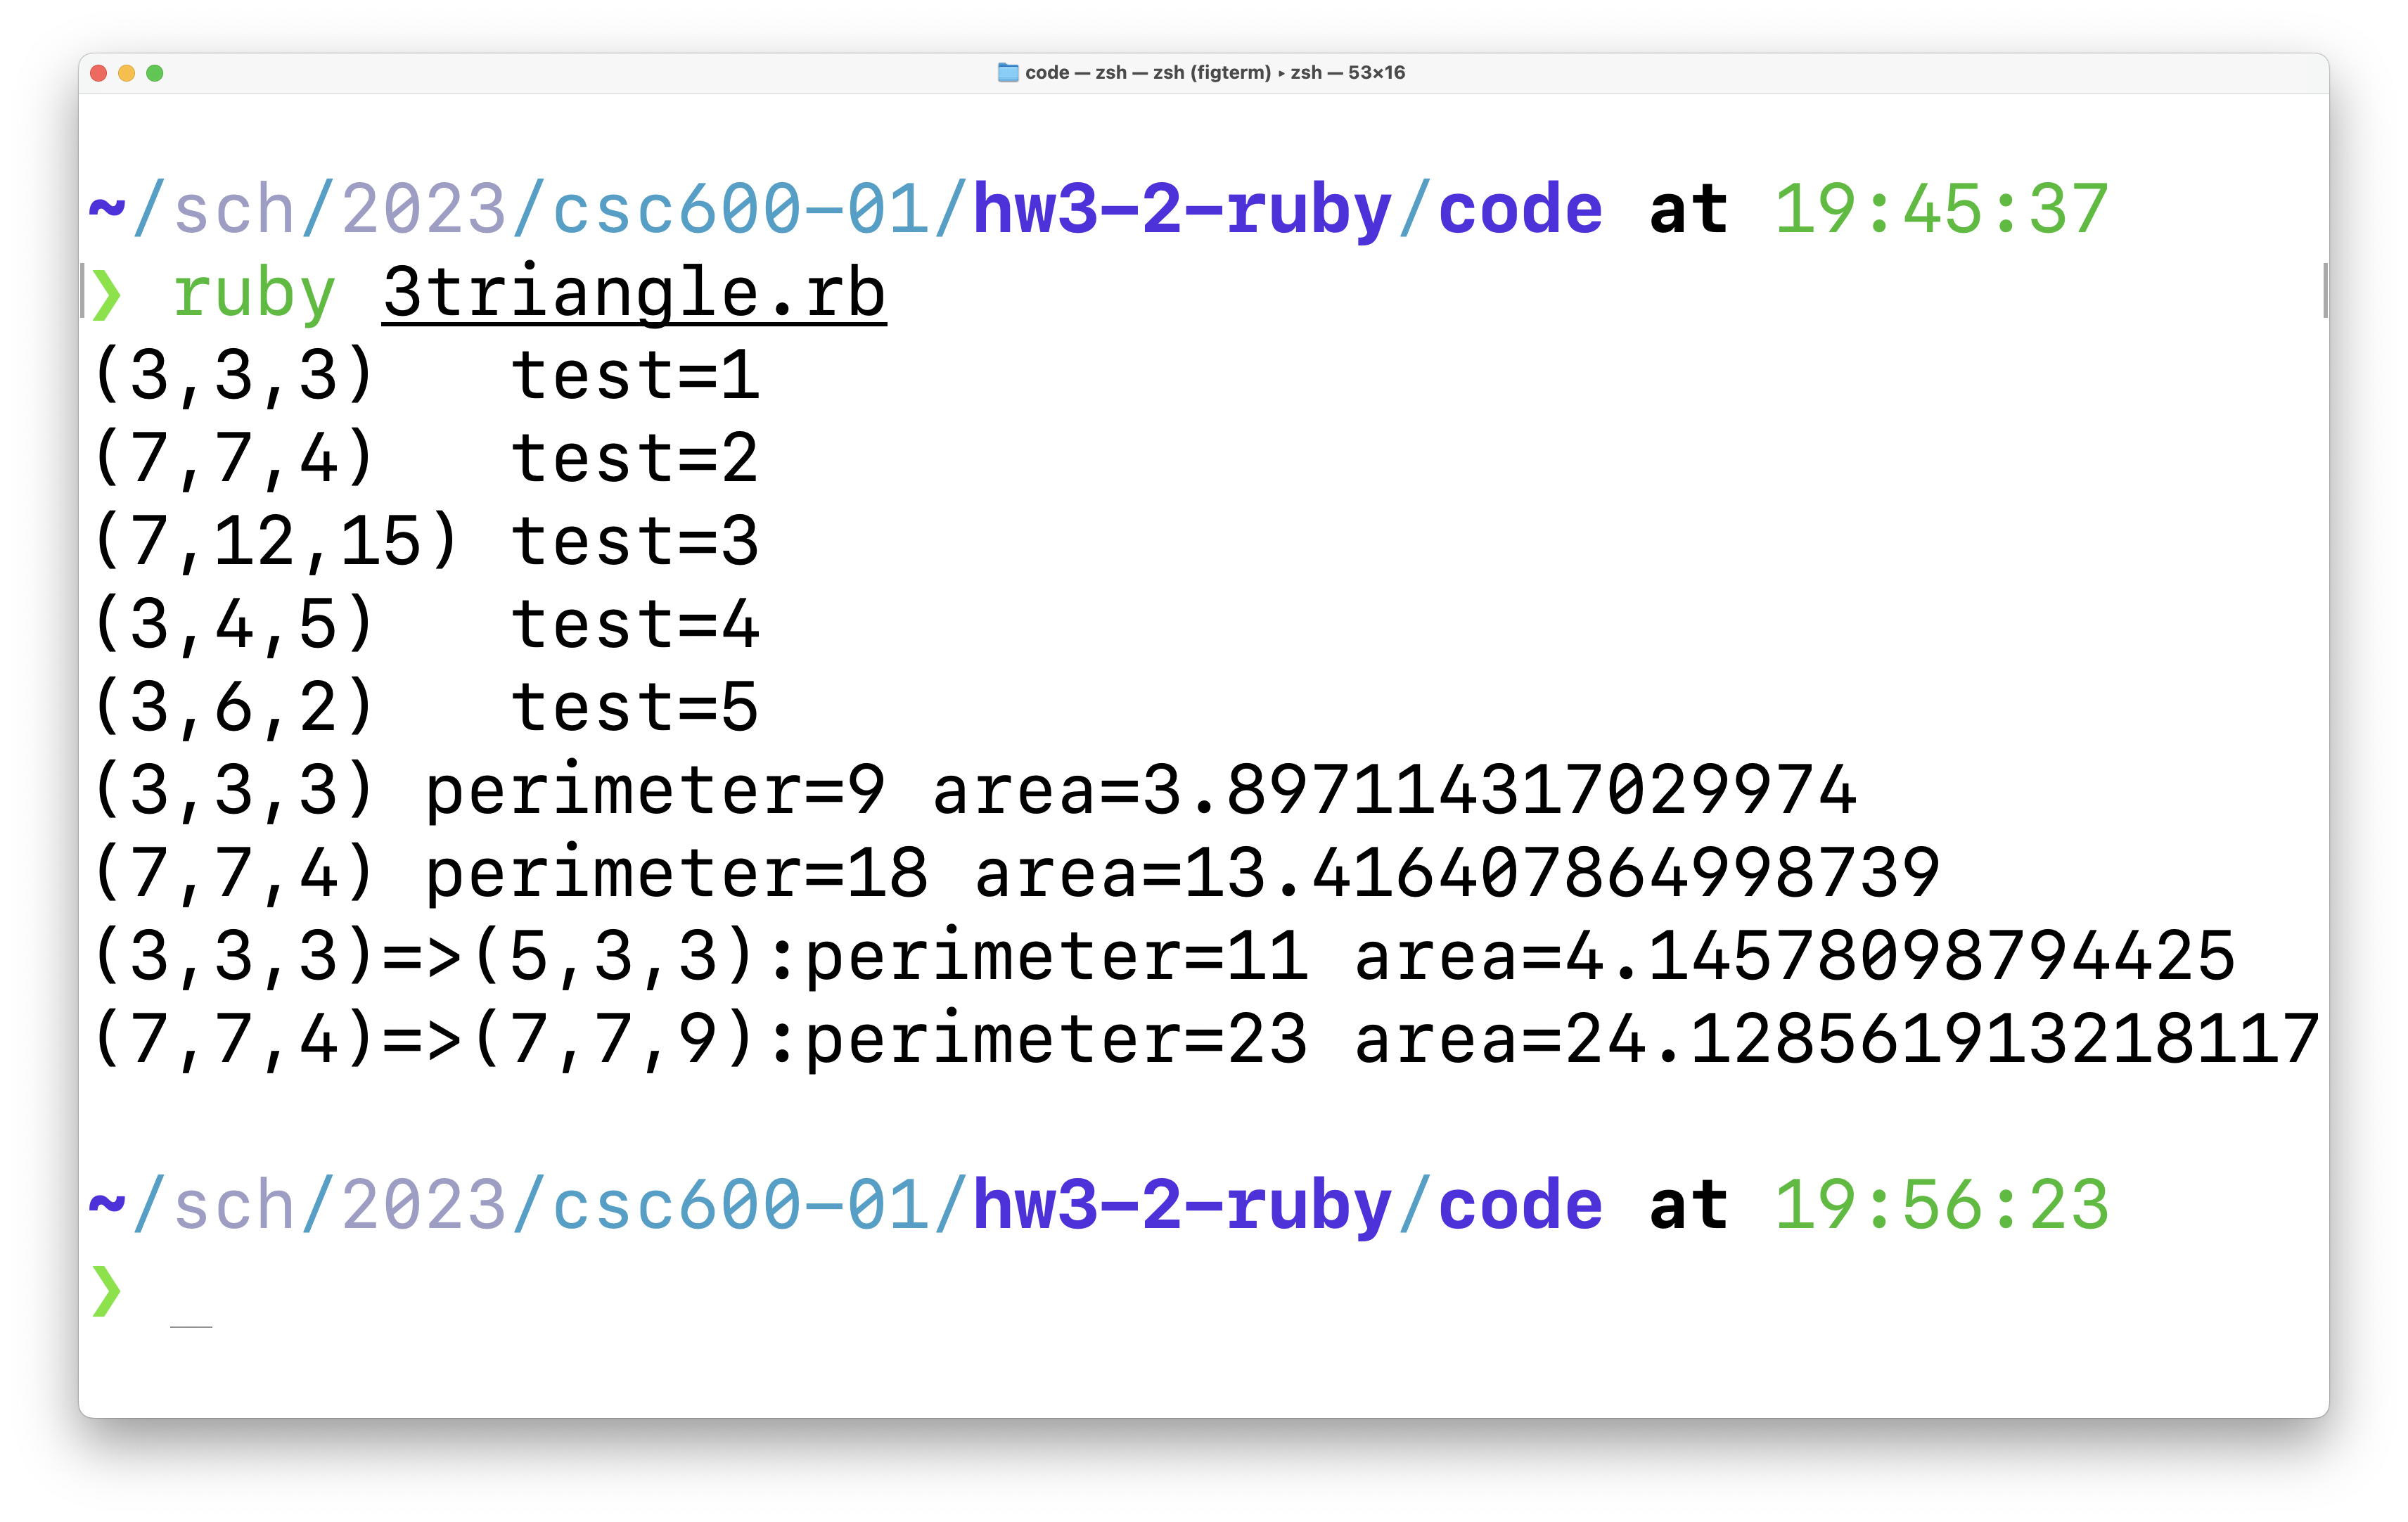
\includegraphics[height=.6\linewidth]{3triangle.PNG}
  \setlength{\captionmargin}{0pt}
  \caption{Screenshot output of executing \emph{3triangle.rb}}
  \label{fig:3triangle.png}
\end{figure}
\addcontentssubsection{\textbf{Figure \ref{fig:3triangle.png}} Screenshot output of executing \emph {3triangle.rb}} % manually adds this listing to table of contents
